\pdfminorversion=7
\documentclass[12pt]{article}

% === Wiley "Proteins: Structure, Function, and Bioinformatics" -- initial (peer-review) submission ===
% The journal's reference style is AMA (numbered, superscript citations in order of appearance).
% Final camera-ready typesetting uses Wiley's official WileyNJD-v2 class with the [AMA] option; this
% source is a clean, self-contained article-class version compliant with Wiley free-format initial
% submission (double-spaced, line-numbered, AMA-numbered references).
\usepackage[T1]{fontenc}
\usepackage[utf8]{inputenc}
\usepackage{amsmath}
\usepackage{newtxtext,newtxmath}   % Times-like serif text + matching math (Wiley/Proteins house style)
% Keep URLs breakable without requesting the unavailable T1/ntxtt typewriter
% shapes that cause font substitution in the submission PDF.
\usepackage{xurl}
\usepackage{microtype}
\usepackage[margin=1in]{geometry}
\usepackage{setspace}
\doublespacing
\usepackage{lineno}
\usepackage{graphicx}
\usepackage{placeins}
\usepackage{booktabs}
\usepackage{array}
\usepackage{authblk}
\usepackage{caption}
\usepackage[super,sort&compress]{natbib}   % AMA-style numbered superscript citations
\usepackage{nameref,hyperref}
\hypersetup{
  colorlinks=true,
  allcolors=blue,
  pdftitle={Reliability boundaries of protein language model zero-shot variant scores},
  pdfauthor={Zeyu Fu},
  pdfsubject={Reliability atlas of ESM-2 zero-shot mutation-effect scores}
}
\urlstyle{same}
\Urlmuskip=0mu plus 1mu\relax
\emergencystretch=4em   % absorb the occasional long unbreakable token in justified text

\makeatletter
\setlength{\@fptop}{0pt}
\makeatother
\renewcommand{\topfraction}{0.95}
\renewcommand{\bottomfraction}{0.90}
\setlength{\textfloatsep}{12pt plus 2pt minus 2pt}
\setlength{\intextsep}{10pt plus 2pt minus 2pt}
\renewcommand{\textfraction}{0.08}
\renewcommand{\floatpagefraction}{0.75}
\raggedbottom
\widowpenalty=10000
\clubpenalty=10000
\displaywidowpenalty=10000
\brokenpenalty=10000

\setcounter{secnumdepth}{2} % genuine numbered Results and Methods subsections

% Captions carry their own "Fig N." / "Table N." prefix in the source text, so suppress the
% automatic "Figure N:" label to avoid double numbering.
\captionsetup{labelformat=empty,labelsep=none,justification=justified,font=small,skip=5pt}

\title{Reliability boundaries of protein language model zero-shot variant scores}

\author[1]{Zeyu Fu\thanks{Correspondence: \href{mailto:fuzeyu99@126.com}{fuzeyu99@126.com}. ORCID: 0009-0001-8329-0108}}
\affil[1]{State Key Laboratory of Trauma and Chemical Poisoning, Institute of Combined Injury, Chongqing Engineering Research Center for Nanomedicine, College of Preventive Medicine, Army Medical University, Chongqing, China}

\date{}
% Generated from clinical-unified/summary.json; do not hand edit.
\newcommand{\ClinicalMacroAUC}{0.7841}
\newcommand{\ClinicalMacroLow}{0.7428}
\newcommand{\ClinicalMacroHigh}{0.8238}
\newcommand{\SigmoidECE}{0.2563}
\newcommand{\SigmoidBrier}{0.2079}
\newcommand{\SigmoidLogLoss}{0.6136}
\newcommand{\PlattECE}{0.0211}
\newcommand{\PlattBrier}{0.1412}
\newcommand{\PlattLogLoss}{0.4441}
\newcommand{\IsoECE}{0.0083}
\newcommand{\IsoBrier}{0.1407}
\newcommand{\IsoLogLoss}{0.4445}
\newcommand{\PooledPrevECE}{0.0000}
\newcommand{\PooledPrevBrier}{0.1808}
\newcommand{\PooledPrevLogLoss}{0.5475}
\newcommand{\GenePrevECE}{0.0100}
\newcommand{\GenePrevBrier}{0.1517}
\newcommand{\GenePrevLogLoss}{0.4657}


\begin{document}

\begingroup
\singlespacing
\maketitle
\endgroup
\linenumbers

\noindent\textbf{Author-review revision, 23 September 2026 --- not submission-ready.}
Corrected row-level clinical scores have been recovered and discrimination,
calibration and uncertainty recomputed from one score version. Independent
scientific review and final visual acceptance of this revision remain open.

\begin{abstract}
\begin{spacing}{1.15}
\noindent Protein language model (PLM) zero-shot variant-effect scores are often treated as general predictors despite task-specific evidence and incompatible score transforms. We audit raw ESM-2 log-likelihood ratios across six axes, with uncertainty where the evidence permits it and applicability-gated controls. Deep mutational scanning (DMS) discrimination rose to a protein-mean area under the receiver operating characteristic curve (AUROC) of 0.725 at 650M parameters, with no detected gain at 3B (paired difference $-0.00015$, 69 proteins, 95\% confidence interval, CI, $[-0.01340,0.01683]$); ProtBERT reached 0.711. Recomputed scores for 4,677 ClinVar variants give a mean AUROC of \ClinicalMacroAUC{} across 20 genes (gene-resampling CI $[\ClinicalMacroLow,\ClinicalMacroHigh]$). On the same scores, five-fold Platt and isotonic calibration yield Brier scores \PlattBrier{} and \IsoBrier{}, compared with \GenePrevBrier{} for a fitting-fold gene-prevalence baseline. Identity-grouped refitting supports these within-panel differences but does not establish transport to new genes or populations. The likelihood readout was a weak stability proxy. Saved antibody--antigen summaries give Spearman approximately 0.08 ($n=627$), but their interval provenance is not fully reconciled and does not support a significance claim. No Benjamini--Hochberg-significant association was detected for polyreactivity (0/14 datasets) or aggregation (0/7). These results support a bounded task-specific audit, not a universal reliability rule or a clinically deployable probability model.

\end{spacing}
\end{abstract}

\noindent\textbf{KEYWORDS:} protein language models, zero-shot variant effect, reliability audit, ESM-2, benchmarking

\bigskip

\section*{Plain-language significance}


Protein language models (PLMs) can rank mutations without labelled training for a particular protein. We examine how far one widely used likelihood score, ESM-2, supports different biological uses. The retained evidence supports mutation-effect ranking in the studied DMS panel, while antibody-binding and developability readouts are weaker and do not support a universal prediction rule. Recovered scores now connect clinical ranking and calibration on the same 4,677 variants. Calibrated probabilities improve proper scoring rules within this gene panel, but this does not show that they remain calibrated in new genes, populations or clinical settings. The research direction remains a task-specific audit, with those limits reported alongside supported findings.


\section{Introduction}

Self-supervised protein language models (PLMs) assign a likelihood to every amino acid in context, and the change in that likelihood when a residue is substituted --- the log-likelihood ratio (LLR) --- is a zero-shot estimate of mutational effect \citep{Meier2021,Rives2021}. Because the estimate requires no labelled training for the target protein, it has been adopted as a general-purpose variant-effect predictor: for deep-mutational-scan (DMS) fitness \citep{Fowler2014,Riesselman2018}, for clinical pathogenicity, for stability and binding changes, and for antibody engineering. The appeal is generality; the risk is that generality is mistaken for uniform reliability. The protocol is uniform across the studied tasks; reliability is task-dependent.

Two problems make the reliability of these scores hard to read from the literature. First, scoring conventions differ --- masked-marginal versus wild-type-marginal LLR, raw scores versus per-assay rescaled or clamped "confidence," different precisions and sequence-length handling --- and these conventions can manufacture apparent differences larger than the real signal. Second, de-circularization is uneven: the same foundation model is pretrained on essentially all natural sequences, so a "held-out" protein family or a curated clinical label is rarely out-of-distribution (OOD) in the way an OOD claim implies, and controls intended to remove a confound are sometimes inapplicable to the very datasets on which they are run.

We therefore do not propose a new model or a new state-of-the-art number. We propose a boundary atlas: a single model family (ESM-2 \citep{Lin2023}, with one cross-family encoder check) evaluated across six decision axes under one fixed discipline. Scores are always the raw LLR, never a clamped or per-assay-rescaled transform. Uncertainty is estimated at the relevant biological unit where the available observations support resampling; point estimates and interval estimates remain distinct. Each de-circularization control is in turn checked for applicability --- defined variance and non-collinearity --- before its verdict is trusted, and claims that fail this check are withdrawn rather than reported. The questions are deliberately operational: how large does the model need to be; is the signal specific to one architecture; does it discriminate curated clinical labels within the studied genes; is it calibrated for stability; does it see binding interfaces; and is it usable for antibody developability. The contribution is the map and the protocol that produces it --- including a record of the over-claims the protocol caught in our own hands.

\section{Results}

Table~\ref{tab1} defines the six task axes, sampling frames, scoring
conventions and native readouts used below. These axes are not independent
replications on a common physical scale.

\begin{table*}[!htbp]
\centering
\caption{{\bf Table 1.} Data, models, and analysis design. ProteinGym scale corroboration uses 217 assays attempted, 201 scored after QC, and 173 proteins on the same panel.}

\label{tab1}
\small\singlespacing
\setlength{\tabcolsep}{4pt}
\begin{tabular}{>{\raggedright\arraybackslash}p{0.225\textwidth} >{\raggedright\arraybackslash}p{0.225\textwidth} >{\raggedright\arraybackslash}p{0.225\textwidth} >{\raggedright\arraybackslash}p{0.225\textwidth}}
\toprule
\textbf{Axis (finding)} & \textbf{Data and labels} & \textbf{Model(s) and scoring} & \textbf{Primary readout} \\ \midrule
Scale (N1) & ProteinGym DMS \citep{Notin2023} (217 assays attempted; 201 scored after quality control, QC; 173 proteins; 79,220 variants); 69-protein de-pseudo-replicated subset & ESM-2 35M/150M/650M/3B, masked-marginal LLR & per-protein AUROC vs size \\
Architecture (N5) & Same 69-protein subset & ProtBERT vs ESM-2 650M, raw LLR & protein-mean AUROC; per-protein Spearman \\
Clinical (N6c) & 4,677 ClinVar variants \citep{Landrum2018}, 20 genes; gnomAD historical sensitivity \citep{Karczewski2020} & ESM-2 650M, recovered fp32 LLRs & AUROC; OOF calibration \\
Stability (N10) & MegaScale single-mutant $\Delta$$\Delta$G \citep{Tsuboyama2023}; \mbox{ThermoMPNN} \citep{Dieckhaus2024} 25\%-id clusters & ESM-2 650M LLR, homology-held-out split & calibration-RMSE inflation (stable-but-weak) \\
Binding (N4) & SKEMPI v2 \citep{Jankauskaite2019} single mutations, 3,424 validated & ESM-2 650M LLR (3B sensitivity) & Spearman(LLR, $-$$\Delta$$\Delta$G) by subset \\
Developability (N9) & FLAb antibody datasets \citep{Chungyoun2024FLAb} (63), 7 properties & ESM-2 650M naturalness & per-property significant fraction \\
\bottomrule
\end{tabular}
\end{table*}



Figures separate task outcomes, sensitivity checks and historical evidence. Figure 1 shows model scaling and scoring-convention sensitivity. Figure 2 uses recovered clinical scores and newly generated per-gene intervals; its gnomAD comparator is historical summary-only. Figure 3 evaluates the same clinical scores with fitting-fold-only probability maps and prevalence baselines. Figures 4--5 examine stability and binding; Figure 6 separates discoveries from control applicability. Figure 7 retains task-specific units and uses the new clinical gene-mean interval. Supplementary figures S1--S9 and Tables S1--S2 preserve the stated evidence-version boundaries.

\subsection{No detected 3B discrimination gain over 650M on this panel}

Across a de-pseudo-replicated 69-protein ProteinGym subset (80 assays attempted; 79 scored after quality control, QC), ESM-2 masked-marginal discrimination of DMS fitness rises from 35M to 650M, with no detected further gain at 3B (Fig 1A). All values are read off the \textit{raw} masked-marginal score, not the clamped per-assay confidence --- the distinction is load-bearing here (see the toolkit-gap correction below): raw-score protein-mean area under the receiver operating characteristic curve (AUROC) is 0.667 at 35M, 0.710 at 150M and 0.725 at 650M, and 3B also rounds to 0.725. The paired, equal-protein difference is $-0.00015$ (3B minus 650M; 10,000-bootstrap 95\% confidence interval, CI, $[-0.01340,0.01683]$), so no gain is detected. On the full ProteinGym benchmark (217 assays attempted; 201 scored after QC, 173 proteins, 79,220 variants), the corresponding 650M masked-marginal result is 0.696 (152/173 proteins above chance; 87.9\%); the WT-marginal sensitivity analysis is 0.702 (150/173; 86.7\%). We therefore retain 650M as the smaller tested model with no detected discrimination loss relative to 3B on this subset; this does not establish equivalence, a universal scaling ceiling or the absence of a meaningful gain on another task. The full-panel result is similar under the two named scoring conventions.

\begin{figure}[!htbp]
\centering
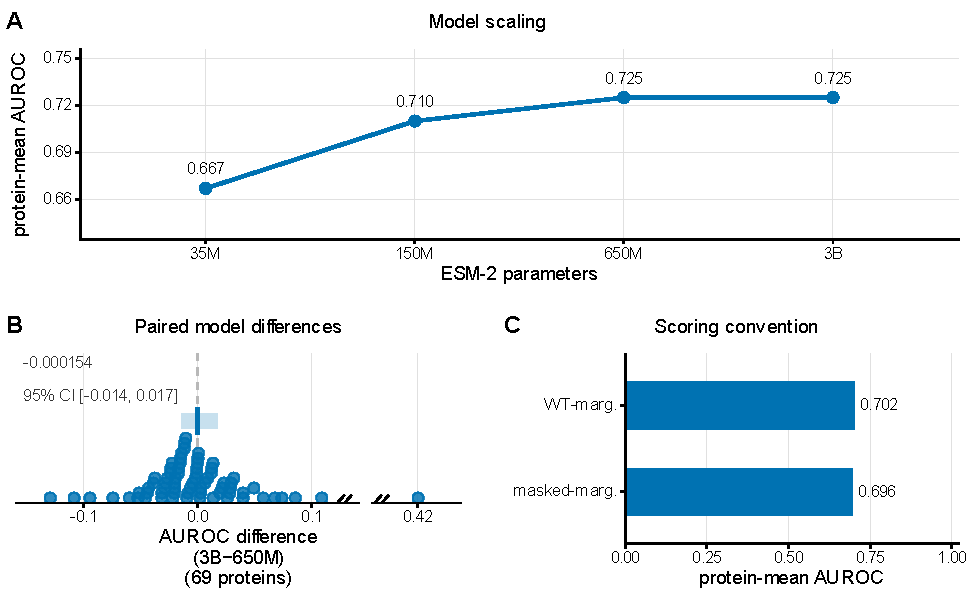
\includegraphics[width=\linewidth,height=0.70\textheight,keepaspectratio]{figures/F1_scale_plateau.pdf}
\caption{{\bf Fig 1. No detected 3B discrimination gain over 650M on the studied protein panel.} (A) ESM-2 masked-marginal protein-mean AUROC across four model sizes on 69 proteins (80 assays attempted; 79 scored). Per-size intervals are unavailable. (B) The paired 3B-minus-650M AUROC differences, with mean $-0.000154$ and a fixed-seed, 2,000-replicate protein-bootstrap 95\% CI $[-0.014,0.017]$. The separate prespecified 10,000-replicate interval reported in the text also spans zero. The broken axis retains the extreme protein without compressing the central observations. (C) Scoring-convention sensitivity on the full ProteinGym panel (217 assays attempted; 201 scored; 173 proteins): masked-marginal 0.696 and WT-marginal 0.702, a difference of 0.006495 before rounding. These two aggregate rows do not supply a paired interval. The result supports no detected gain at 3B on this subset, not equivalence or a universal scaling law.}

\end{figure}


This conclusion survived a methodological correction that is itself part of the result. An earlier version of this axis reported a "toolkit reproducibility gap" ($\approx$0.05 AUROC) and a "masked beats wild-type" advantage; both vanished when scores were read off the raw LLR rather than a min--max-clamped confidence (raw gaps $-$0.003 and $-$0.005). The clamped transform had manufactured rank differences larger than the real effect. The saved tier and coverage comparisons show why this transform is unsuitable for selective ranking (Fig.~S4A--D). The distinct position-held-out assay study retains its own test set and pooled readout (Fig.~S1A--C).

In that separate position-held-out study, 19 assays contribute 1,551 test
variants, pooled AUROC is 0.781 and 13 of 19 saved assay intervals exclude
chance (Fig.~S1A--C). These are not extra observations for the 69-protein
scale comparison. The full-, confidence-selected- and shuffled-coverage
views in Fig.~S4 reuse the archived tier records; they do not supply
tier-specific resampling uncertainty or a validated abstention policy.

\subsection{The signal is shared across masked-LM encoders}

To test whether the variant-effect signal is a property of ESM specifically or of masked-language modelling more broadly, we scored the same proteins with ProtBERT \citep{Elnaggar2021}, a BERT-family encoder trained on a different corpus (UniRef100+BFD) with different architectural details (Fig~S6A--D). ProtBERT reaches protein-mean AUROC 0.711, comparable to ESM-2 650M (0.725 masked, 0.728 wild-type), and the two models agree moderately on which proteins are easy versus hard (per-protein Spearman 0.65--0.67; positive but well short of identity); a wild-type-marginal control on ProtBERT reproduces the agreement. The agreement is on the aggregate difficulty ranking, not per protein: each encoder rescues a minority of proteins the other scores near chance (in both directions), so per-protein reliability is partly encoder-specific --- which motivates, but does not evaluate, an ensemble; this does not weaken the shared-signal claim, since that rests on comparable mean AUROC and a positive rank correlation rather than on per-protein identity. We scope this carefully: it demonstrates robustness across independently trained MLM \textit{encoders}, not independence from broad architecture classes --- autoregressive PLMs and structure-conditioned models are untested. ProtBERT's small mean deficit ($\approx$0.014) is consistent with it being an older, smaller model, not with an architecture-class difference. A second, independent ESM training run (ESM-1v, a different pretraining recipe on the same UniRef family) gives the same picture on the full 217-assay benchmark --- protein-mean AUROC 0.711 versus ESM-2's 0.702, with a per-protein Spearman of 0.73 --- so the signal is also stable across ESM training runs, not an artifact of one set of weights (though ESM-1v was itself purpose-trained for variant effect, so this is stronger evidence against a single-weights artifact than it is evidence of task-generic architecture independence). Externally, the zero-shot signal is also competitive with established variant-effect predictors: on the Livesey \& Marsh deep-mutational-scanning compilation (10 proteins with overlapping coverage), ESM-1v's per-protein rank agreement with DMS (median $|\rho| = 0.49$) is at the top of a panel that includes EVE (0.35), DeepSequence (0.45) and the supervised predictors REVEL (0.47), VESPA (0.40) and CADD (0.37) (Fig S5A--D) --- so the moderate discrimination we report is not an ESM-specific weakness but the achievable level for a single sequence-only zero-shot pass on this task. Broad benchmark resources (FLIP and FLAb), evolutionary generative predictors such as EVE, and isoform-aware ESM1b variant-effect prediction are complementary evaluation or modelling settings, not evidence that this single-model atlas has measured their performance \citep{Dallago2021FLIP,Chungyoun2024FLAb,Frazer2021EVE,Brandes2023ESM1b}. We scope the word ``achievable'' carefully: it marks what one sequence-only base model reaches, not an intrinsic ceiling of protein representation, since recent methods lift variant-effect discrimination beyond any single base model --- by co-distilling the collective knowledge of the ESM family into one sequence-only model \citep{Dinh2026VESM} or by adding a structure-aware token vocabulary \citep{Su2024SaProt} --- design spaces this single-model, sequence-only audit deliberately does not cover.

The named Livesey--Marsh comparison uses the published DMS compilation rather than a dataset reconstructed for this audit (Fig.~S5A--D) \citep{Livesey2020}.
EVE has coverage for seven proteins while the other displayed predictors
have ten (Fig.~S5D), so the unpaired descriptive medians do not establish
a universal predictor ordering. Likewise, the AUROC and agreement views
in Fig.~S6 reuse the same 69 proteins rather than adding four independent
encoder experiments.

\subsection{Clinical discrimination from a recovered, identified score table}

The revised clinical analysis uses one row-level table of 4,677 identified
ClinVar variants across 20 genes. Complete official ESM-2 650M weights were
loaded in fp32, and wild-type-marginal LLRs were recomputed from the validated
reference sequences. All 24 full-sequence and windowed AUROCs reproduced the
saved corrected N6c summaries to their four-decimal precision. Repeated
full-sequence forwards were bitwise identical for all 20 genes in this run.
These are newly recovered scores, not scores inferred from AUROC targets.

Using the stated primary score (mutation-centred windows for sequences
longer than 1,024 residues), the mean per-gene AUROC is
\ClinicalMacroAUC{} (gene-resampling 95\% interval
$[\ClinicalMacroLow,\ClinicalMacroHigh]$; range 0.5571--1.0000).
Sixteen of 20 point estimates are at least 0.70 (Fig.~2).
Per-gene whiskers now use 2,000 class-stratified variant bootstrap draws,
replacing the unsupported historical intervals. For AICDA, perfect
separation of the 24 observed variants gives the expected empirical interval
$[1,1]$; this is not evidence of zero population uncertainty.
The saved gnomAD benign-source comparison remains a separately labelled
summary-level sensitivity (Fig.~2B and Fig.~S2). Its population-control
variants were not rescored in this revision. Gene exposure in sequence
pretraining and clinical ascertainment limit all of these comparisons to
the studied panel. Its saved mean gnomAD-minus-ClinVar AUROC difference is
$-0.019565$ (Fig.~S2); without paired uncertainty or newly recovered gnomAD
rows, this is a benign-source sensitivity, not a causal ascertainment
effect or transport test. The recovered table contains 1,108 pathogenic
and 3,569 benign variants; per-gene calibration bins, Brier scores and log-loss values
for these same rows are retained in the reproducibility exports accompanying
SI Table~S1. The discrimination and calibration results therefore refer to
one identified score version rather than to separate historical summaries.

\begin{figure}[!htbp]
\centering
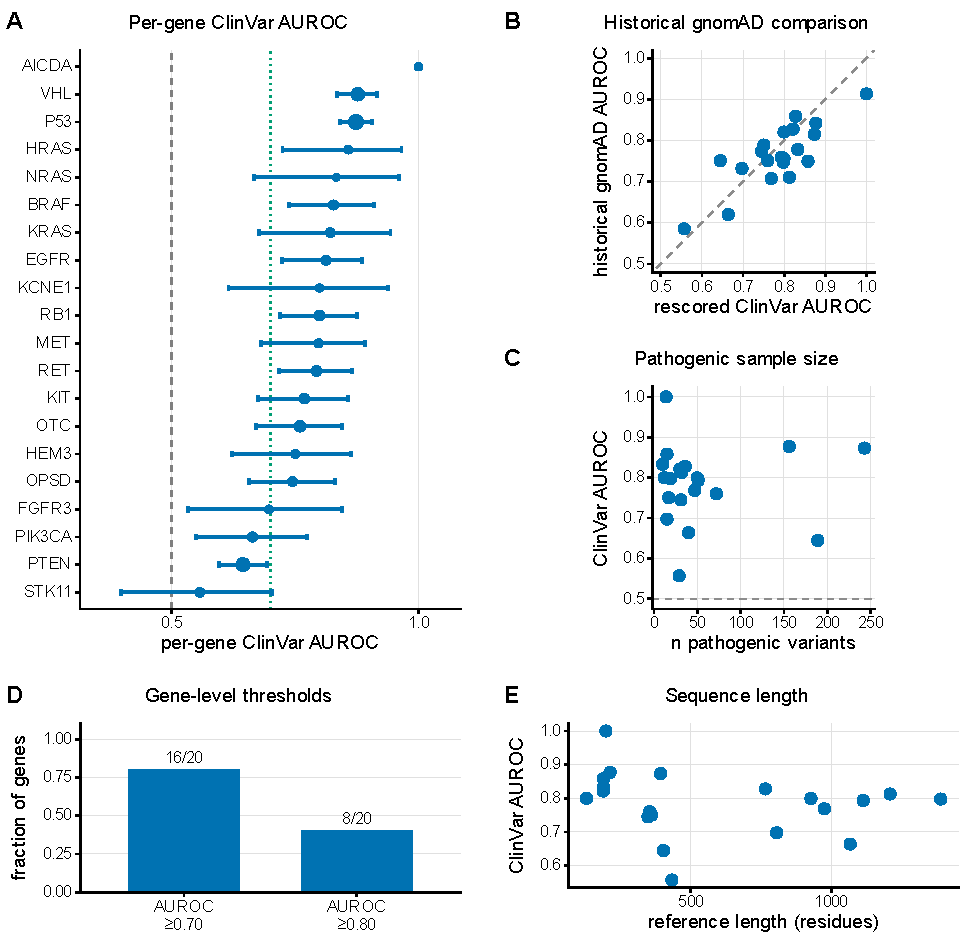
\includegraphics[width=\linewidth]{figures/F3_clinvar_forest.pdf}
\caption{{\bf Fig 2. Clinical discrimination from recovered fp32 scores.} (A) Per-gene AUROC for 4,677 variants across 20 genes, with 95\% percentile intervals from 2,000 class-stratified variant bootstrap draws; marker size indicates pathogenic sample size. AICDA's empirical interval is $[1,1]$ under perfect observed separation, not a claim of zero population uncertainty. Dashed and dotted lines indicate 0.5 and 0.70. (B) Newly recovered ClinVar AUROC versus the historical gnomAD-benign summary, not a newly rescored gnomAD cohort. (C) AUROC versus pathogenic sample size. (D) Point-estimate thresholds, 16/20 at AUROC $\geq0.70$ and 8/20 at $\geq0.80$. (E) Reference-sequence length versus AUROC. The new intervals are unadjusted per-gene summaries; no simultaneous significance or clinical-transport claim is made.}

\end{figure}

\subsection{Same-score calibration improves proper scores within the panel}

We next calibrated the same recovered LLRs with five-fold, class-stratified
cross-fitting, estimating all standardization and probability maps from
the fitting folds only. The sigmoid of the standardized negative LLR is
an arbitrary comparator, not a native model probability. Its pooled ECE
is \SigmoidECE{} and its Brier score is \SigmoidBrier{}.
Pooled Platt and tie-invariant isotonic maps reduce ECE to \PlattECE{}
and \IsoECE{}, with Brier scores \PlattBrier{} and \IsoBrier{}
(Fig.~3; Table~S1). Corresponding log losses are \PlattLogLoss{}
and \IsoLogLoss{}; the smaller isotonic ECE does not establish overall
superiority over Platt.

The fitting-fold pooled-prevalence baseline has ECE below $10^{-6}$ despite
a Brier score of \PooledPrevBrier{}. Class stratification makes that
near-zero pooled ECE unsurprising. A gene-prevalence baseline has Brier
score \GenePrevBrier{} and log loss \GenePrevLogLoss{}.
Thus low ECE alone does not imply useful variant discrimination. Relative
to this stronger gene-specific baseline, the paired Brier differences are
$-0.0105$ for Platt and $-0.0110$ for isotonic, with identity-grouped
refitting percentile ranges $[-0.0161,-0.0072]$ and
$[-0.0160,-0.0070]$, respectively. These differences support added
within-panel probability information beyond gene prevalence, conditional
on the observed gene and class composition.
The complete map-by-map OOF values and the identity-grouped refit summaries
are given in SI Tables~S1--S2. Table~S2 is part of the result chain because
the original OOF point, bootstrap mean and percentile range answer different
questions; the refit distribution is not a replacement confidence interval
for the fixed-fold point.

\begin{figure}[!htbp]
\centering
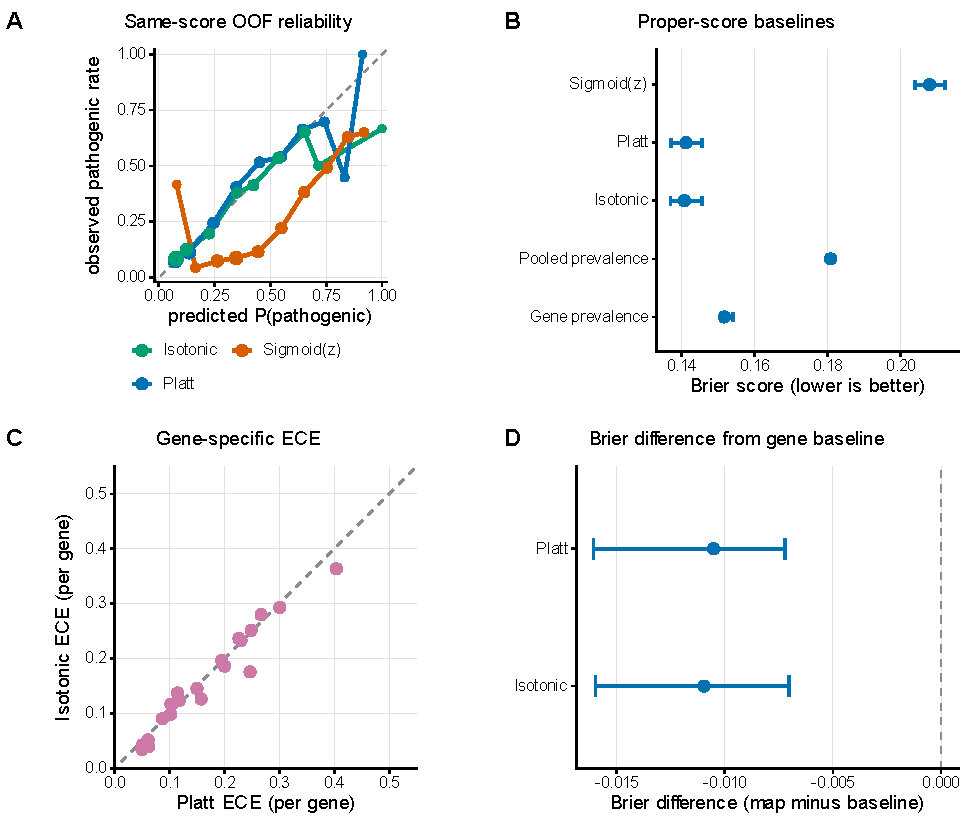
\includegraphics[width=\linewidth]{figures/F4_clinical_calibration.pdf}
\caption{{\bf Fig 3. Same-score, within-panel calibration with explicit baselines.} All panels use five-fold OOF predictions for the same 4,677 variants as Fig.~2 (seed 20260923). Standardization and calibrators use fitting folds only. (A) Ten equal-width reliability bins for sigmoid($z$), pooled Platt and tie-invariant isotonic maps; point size indicates bin count, and only occupied bins are connected. Sigmoid($z$) is not a native model probability. (B) Brier scores, including pooled- and gene-prevalence baselines fitted on the same training folds. (C) Per-gene ECE under the two calibrated maps, using these same OOF predictions; each point is one gene, not an independent calibration experiment. (D) Paired Brier differences from the gene-prevalence baseline. Whiskers in B and D are 2.5th--97.5th percentiles of 1,000 gene-by-class-stratified refitting draws, keeping each original variant in one fold and retaining bootstrap multiplicity. Points and refit distributions are reported separately and need not be centred. These are within-panel results, not gene/position holdout or clinical deployment validation.}

\end{figure}

\subsection{Uncertainty and version boundaries limit the clinical claim}

The 1,000 refitting draws resample within gene and class and preserve each
original variant's multiplicity without splitting its copies across
fitting and evaluation folds. This corrects bootstrap-copy leakage, but
is not a gene-, residue-position- or homology-disjoint evaluation. Pooled
calibration also does not guarantee calibration for each gene (Fig.~3C).
The percentile ranges describe the refitted bootstrap distribution, not
intervals centred on a fixed-fold point. For example, isotonic ECE is
0.0083 on the original OOF predictions, whereas its refit mean is 0.0159
and its 95\% percentile range is $[0.0090,0.0253]$. The difference is
reported rather than shifting the interval to include the point. The
first-half and second-half Monte Carlo ranges are retained in SI Table~S2,
and the per-gene reliability-bin coordinates are retained in the exports
used for Fig.~3. These supplemental records do not add a new clinical
population: they document the same 4,677 identified variants and the same
within-panel estimand.

The old calibration table had a mean per-gene AUROC of 0.6560, compared
with 0.7841 for the corrected scorer. Its six-gene reliability figure,
twenty-gene degradation counts, Cox/Holm analyses, selective-prediction
claims and decision-curve conclusions are not carried forward. They
remain historical audit records. The revised figures, intervals and
proper-score comparisons all derive from the recovered table.
Exploratory coverage and decision-curve coordinates are retained in the
reproducibility data, but do not establish a clinically chosen threshold,
external calibration or deployment benefit. Independent clinical
validation remains necessary.


\subsection{A weak fold-stability proxy and an interface-ranking abstention}

Two stability/binding axes locate where the zero-shot score's physical meaning ends. Protein stability is a \textit{stable-but-weak} proxy. On the clean cluster-disjoint homology-held-out split (MMseqs2 25\%-identity clusters), held-out calibration-RMSE inflation is 0.037--0.039 and discrimination is similar between the training and held-out partitions (Fig 4A--C). We deliberately do not read this as a passed out-of-distribution falsification test: for a model pretrained on essentially all natural sequences a homology-held-out split is not genuinely out-of-distribution, and the absence of a gap cannot by itself establish independence from pretraining exposure. The load-bearing observation is instead that the signal is weak everywhere (Spearman 0.358--0.384, well below the published ThermoMPNN literature range 0.6--0.7, which is not a paired audit on this split) and that absolute calibration RMSE stays high (0.911--0.951 on $n_{\mathrm{train}}=164{,}094$ / $n_{\mathrm{held-out}}=42{,}563$ mutations; 66/26 clusters) --- a stable but low-ceiling proxy. A superseded v1 split contained four overlapping clusters (55,592 held-out mutations; 66/30 clusters) and is retained only as a provenance audit, not as headline evidence.

\begin{figure}[!htbp]
\centering
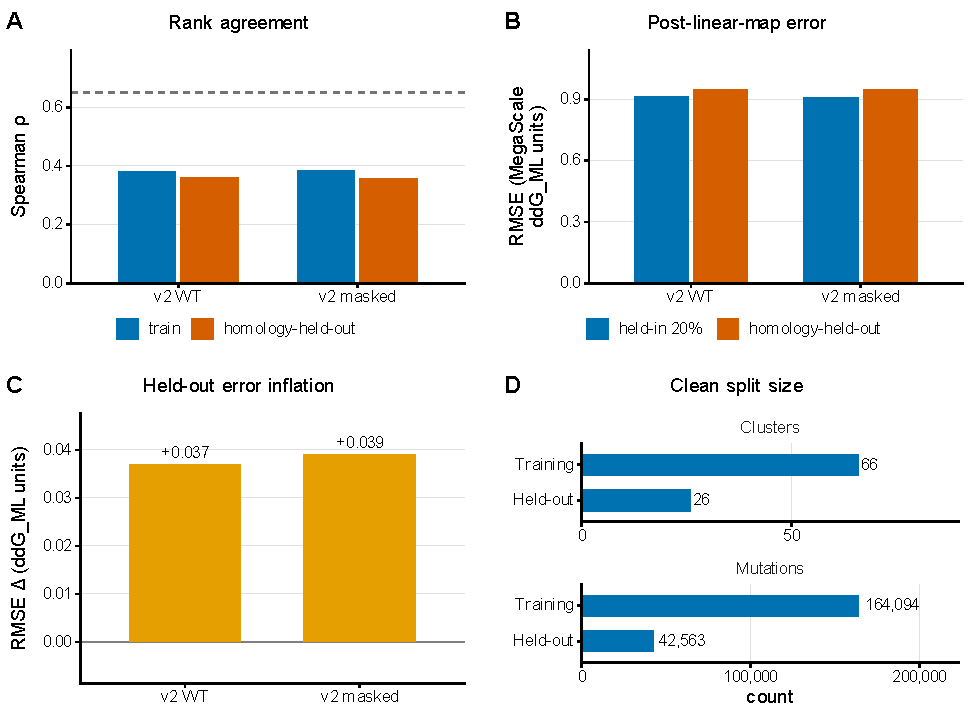
\includegraphics[width=\linewidth,height=0.70\textheight,keepaspectratio]{figures/F5_stability_ddg.pdf}
\caption{{\bf Fig 4. Stability readouts on a clean homology holdout.} (A) Raw-score Spearman correlation for WT- and masked-marginal scoring in training and homology-held-out mutations. The dashed ThermoMPNN value near 0.65 is a literature reference, not a paired estimate. (B) RMSE after a linear map fitted to 80\% of training mutations, evaluated on the held-in 20\% and homology-held-out mutations. Units are dataset-native MegaScale \texttt{ddG\_ML}; fitted coefficients were not retained. (C) Held-out-minus-held-in RMSE differences, 0.037 and 0.039. (D) Mutation and sequence-cluster counts in separate, labelled scales: 164,094 and 42,563 mutations; 66 and 26 clusters. The clean split excludes overlapping clusters. Across the two scoring conventions, the saved mean Spearman difference is $-0.0225$ and the mean RMSE difference is 0.0385; neither supplies a cluster-bootstrap interval. The readout is a descriptive stability proxy, not a deployable calibration or pretraining-independent validation.}

\end{figure}


A separate supervised analysis evaluates uncertainty from frozen PLM embeddings under distribution shift (Fig.~S7A--D). The saved uncertainty--error associations vary by method and split. The BayesianRidge acquisition record contains a higher UCB final-best label on the GB1 low-versus-high split (7.2287 versus 6.2911); the other displayed UCB and greedy entries coincide. A separate cache-based aggregate records zero UCB wins. These are different provenance paths and cannot support a universal ``never beats greedy'' statement. We therefore display the per-split acquisition observations with separate dataset-native axes, omit the conflicting win-count comparison, and make no general acquisition-utility claim. No cross-dataset average of fitness and temperature outcomes is interpreted as a physical effect.

For protein--protein binding $\Delta$$\Delta$G (SKEMPI v2, 3,424 validated single mutations) the correlation is stratified, not a judged collapse law (Fig 5C). The overall prespecified LLR readout correlates weakly with destabilization (Spearman 0.20, 95\% CI $[0.167, 0.231]$); that observation does not identify what interface information may exist elsewhere in the model representation. Figure 5A--B connects the binding readout to a deposited hormone--receptor complex and two same-site substitutions from the existing sensitivity table; Fig 5D displays their 3B scores. These illustrative cases do not establish a conformational mechanism. Subset counts are two partitions of that same $3{,}424$, not two experiments (Table 2): partition A is antibody--antigen ($n=627$) versus all remaining mutations labelled general/non-antibody ($n=2{,}797$; $2{,}797+627=3{,}424$); partition B is structural interface ($n=2{,}792$) versus non-interface ($n=632$; $2{,}792+632=3{,}424$). The $n=2{,}797$ and $n=2{,}792$ figures are different subset definitions, not a five-mutation discrepancy. The diagnostic contrast used here is partition A: general/non-antibody mutations hold at 0.22 (95\% CI $[0.185, 0.258]$, $n=2{,}797$) while the archived antibody--antigen estimate is approximately 0.08 ($n=627$). The N4 summary retains interval $[0.002,0.157]$, but the separately archived antibody-language-model comparison retains $[-0.0022,0.1597]$ for its ESM-2 entry (Fig.~S8). The row/scorer/resampling identities of these summaries are not reconciled here; similar points and denominators do not prove equivalence. We make no significance, subgroup-difference or interface-boundary claim from that discrepancy. Non-interface positions sit at $\approx$0 ($n=632$), corroborative only because their narrow binding-$\Delta$$\Delta$G range restricts Spearman regardless of model quality. A mean-LLR gradient from gain-of-binding through neutral to destabilizing mutations is consistent with a coarse destabilization prior, but it cannot establish the internal mechanism; the model-size and scoring-convention sensitivity remains bounded by the subset intervals (Fig.~S3A--D). We therefore do not rely on this LLR readout to rank interface or antibody-binding mutations, while leaving representation-level interface recognition untested.

\begin{table}[!htbp]
\centering
\caption{{\bf Table 2.} SKEMPI v2 single-mutation subset counts are two partitions of one $n=3{,}424$ set, not two experiments. Partition A (antibody--antigen versus all remaining mutations) and partition B (structural interface versus non-interface) each sum to $3{,}424$. Adding $2{,}797+627+632$ would double-count. Interface $n=2{,}792$ is not a five-mutation revision of general/non-antibody $n=2{,}797$. The antibody--structural-interface intersection is a third subset ($n=525$) and is not a row of this table.}

\label{tab2}
\small\singlespacing
\setlength{\tabcolsep}{3pt}
\begin{tabular}{>{\raggedright\arraybackslash}p{0.22\textwidth} >{\raggedright\arraybackslash}p{0.42\textwidth} r >{\raggedright\arraybackslash}p{0.22\textwidth}}
\toprule
\textbf{Subset} & \textbf{Definition} & $\boldsymbol{n}$ & \textbf{Adds to $3{,}424$?} \\
\midrule
overall & all validated SKEMPI v2 single mutations & 3{,}424 & total \\
antibody--antigen & Ab--Ag interface mutations & 627 & partition A with general \\
general (non-antibody) & all mutations that are not antibody--antigen (includes interface and non-interface) & 2{,}797 & A: $2{,}797+627=3{,}424$ \\
interface & structural interface (Ab--Ag plus non-Ab interface) & 2{,}792 & partition B with non-interface \\
non-interface & non-interface positions & 632 & B: $2{,}792+632=3{,}424$ \\
\bottomrule
\end{tabular}
\end{table}

\begin{figure}[!htbp]
\centering
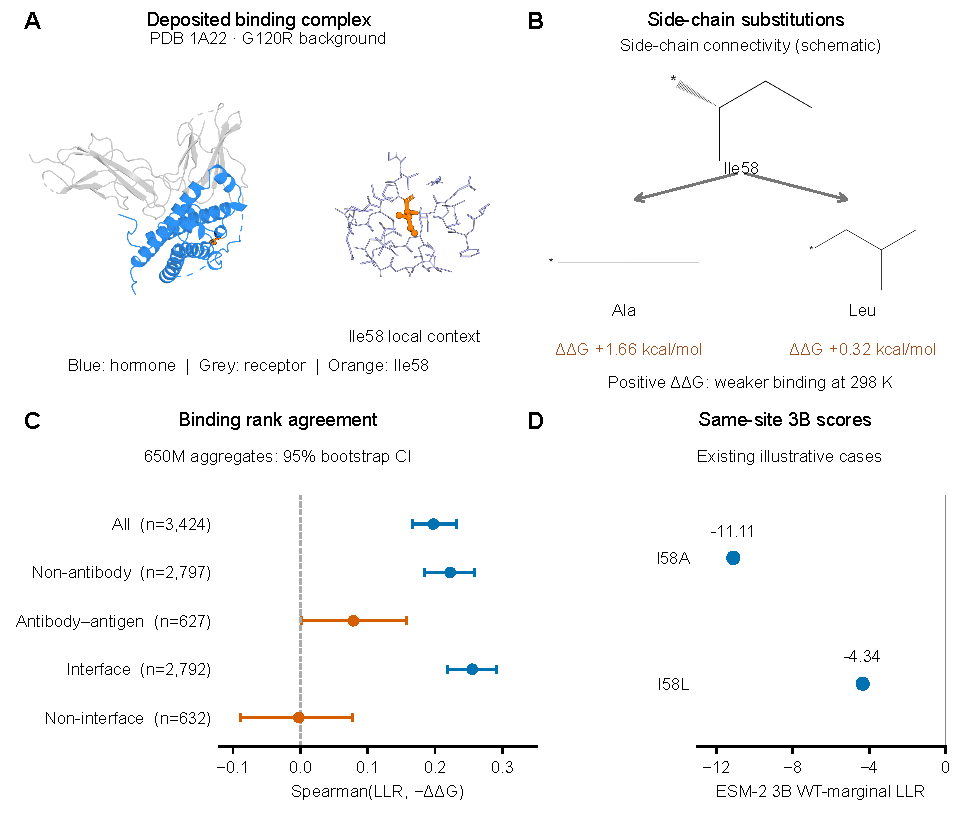
\includegraphics[width=\linewidth,height=0.70\textheight,keepaspectratio]{figures/F7_binding_boundary.pdf}
\caption{{\bf Fig 5. Physical binding changes and the limits of a sequence-likelihood score.} (A) Deposited human growth hormone (blue) bound to its receptor (grey), with Ile58 highlighted in orange and enlarged. The coordinate context is PDB 1A22, which contains the G120R hormone background; it is not a structure of either illustrated Ile58 mutant. (B) Side-chain connectivity for I58A and I58L and their existing SKEMPI-derived binding $\Delta\Delta G$ values at 298 K. Asterisks indicate attachment to the backbone. Positive values denote weaker binding. These are chemical schematics, not inferred mutant conformations. (C) Archived ESM-2 650M aggregate Spearman estimates, denominators and bootstrap intervals from the N4 result summary; antibody and interface subsets are overlapping partitions, not independent experiments. The antibody--antigen interval here differs from the separately archived comparison in Fig S8. Their row/scorer/resampling identity is not reconciled; neither zero-crossing status nor a subgroup difference is promoted as a new test. (D) Existing 3B WT-marginal sensitivity scores for the same two substitutions. The cases illustrate replacements at one mapped site, not predictive performance or a structural mechanism. No new assay, predicted contact change or independent validation is added.}

\end{figure}


\subsection{Antibody developability: liabilities without detected signal}

We map the zero-shot "naturalness" score onto 63 FLAb datasets and seven properties (Fig 6A--B). No BH-significant associations are detected for polyreactivity (0/14 datasets) or aggregation (0/7), after Benjamini--Hochberg control at $q=0.05$ across the full panel. These denominators are insufficient to exclude small $|\rho|$; absence of detection is not equivalence to zero. Non-liability properties are heterogeneous: expression has 4/4 detected associations ($|\rho|$ 0.31--0.48), immunogenicity 1/1, and thermostability 1/4. Expression and immunogenicity are not liability endpoints, and their small dataset counts are not promoted as validated atlas nodes. For binding, 27 of 30 datasets are single-parent DMS designs with constant germline identity. In those designs germline identity has no variance and cannot explain a within-dataset correlation; a germline-distance partial-correlation control is undefined, not evidence that a signal was removed. Fourteen of those 27 datasets have BH-significant raw associations ($|\rho|$ up to 0.69); overall binding has 16/30. This design-specific result does not establish general deconfounding, independence of all other determinants or screening utility. In the three multi-germline datasets, naturalness and germline distance are collinear ($|\rho|$ 0.6--0.86), leaving the partial-correlation analysis underpowered. No FLAb binding dataset supplies a well-powered germline de-circularization test. The earlier "binding is germline-confounded (18$\rightarrow$4)" summary incorrectly coded an inapplicable control as signal loss and is withdrawn. The supported contrast is between endpoint-specific detections and non-detections under these designs, not a validated developability pipeline.

The liability interpretation follows the distinction between sequence-level developability screening and therapeutic-antibody optimization benchmarks \citep{Jain2017,Raybould2019,Hie2024,Shanker2024}; these references motivate the endpoints but do not upgrade the null associations into equivalence claims.

\begin{figure}[!htbp]
\centering
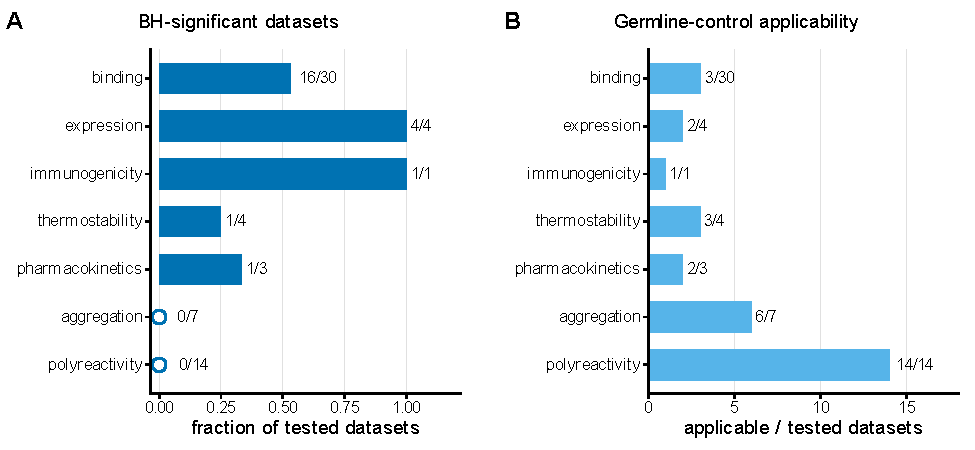
\includegraphics[width=\linewidth,height=0.70\textheight,keepaspectratio]{figures/F8_developability_map.pdf}
\caption{{\bf Fig 6. Discovery and control applicability are distinct quantities.} (A) Fraction of datasets passing Benjamini--Hochberg $q<0.05$ across all 63 FLAb datasets. Every label gives significant/tested counts. Open markers at zero explicitly represent zero detected associations for polyreactivity (0/14) and aggregation (0/7); no data are missing at these positions. (B) Datasets eligible for germline-distance partial correlation, with applicable/tested counts for the same seven properties. Ineligibility is a design restriction, not a failed discovery. Constant germline identity in a single-parent assay cannot support that control. The property-level discovery summaries lack independent effects and variances needed for effect intervals or minimum-detectable-effect estimation. Zero discoveries do not establish absence of an effect or equivalence.}

\end{figure}


Does an antibody-specific likelihood readout provide a different result? The archived AntiBERTy comparison addresses that narrower question (Fig~S8A--D), with the ESM-2 antibody-summary provenance restriction stated above. On aggregation neither likelihood readout has a BH-significant association (0/7 datasets for each); absence of detection does not establish equivalence to zero. For antibody--antigen binding $\Delta$$\Delta$G the archived point estimates are small (AntiBERTy Spearman 0.04 with an interval spanning zero; ESM-2 approximately 0.08). The unresolved ESM-2 row/scorer/resampling identities prevent a validated between-model or zero-effect inference at this node. For polyreactivity the archive records a modest AntiBERTy signal (3/14 versus 0/14 datasets surviving correction, maximum $\rho$ 0.34, with all three detections from one correlated panel), which is not an independent multi-panel validation. The practical reading is therefore readout-specific: neither tested zero-shot likelihood is demonstrated here to be a dependable predictor of these liabilities; whether either model's latent representation contains useful interface information remains untested here.



\subsection{Exploratory descriptors do not establish a transferable reliability predictor}

We explored whether simple task descriptors could anticipate discrimination (Fig.~S9A--D). The saved predictor table contains 69 DMS proteins and 20 ClinVar gene summaries. The strongest reported DMS association, raw-score spread versus AUROC (Spearman approximately 0.25), has a bootstrap interval touching zero. Clinical score spread was missing for all 20 genes in that analysis; its transfer to ClinVar was therefore \textit{not evaluated}, not shown to fail. The recorded DMS multivariable fit used sample size, score mean, score standard deviation and a length proxy, not class balance; its descriptive $R^2$ was approximately 0.03. Length and sample-size associations differed between the available axes, but these small, non-independent task panels do not establish a general sign reversal or a multifactorial mechanism. Alignment depth and positional conservation were not available. The supported conclusion is limited: these exploratory summaries do not establish a transferable reliability predictor. New clinical scores do not retrospectively turn that missing-variable comparison into a completed test.



\subsection{Task-specific reliability synthesis}

The task-level synthesis separates AUROC and Spearman correlations into their own metric panels (Fig.~7A--B). Overlapping binding subsets are not independent tasks, and starred antibody nodes retain their unresolved archive status. We omit the shared null-gap scale and heuristic zone counts so the graphic cannot imply a common physical effect or validated reliability category. The panels reuse the existing study evidence and add no independent replication.

\begin{figure}[!htbp]
\centering
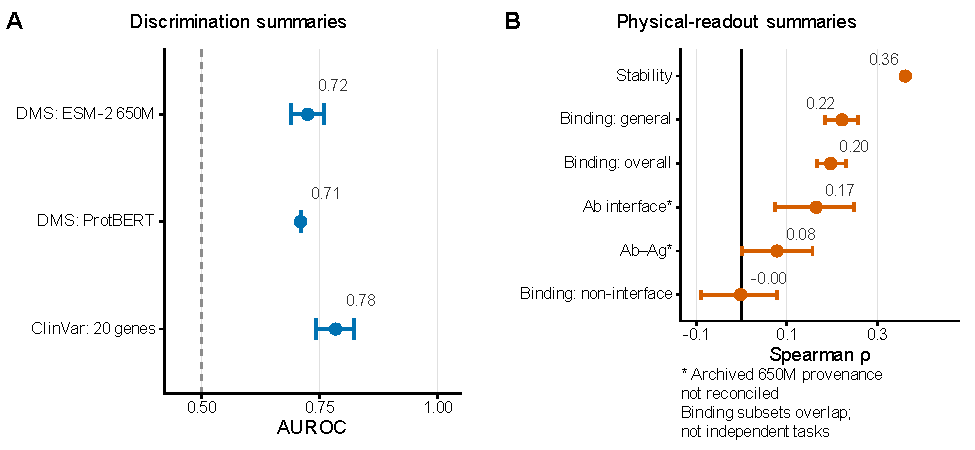
\includegraphics[width=\linewidth,height=0.70\textheight,keepaspectratio]{figures/F11_boundary_atlas.pdf}
\caption{{\bf Fig 7. Task-specific evidence summaries in separate metric units.} (A) AUROC summaries; the ClinVar point and 10,000-draw gene-resampling interval are recomputed from the recovered row-level scores (mean \ClinicalMacroAUC{}, interval $[\ClinicalMacroLow,\ClinicalMacroHigh]$). (B) Saved Spearman summaries for physical readouts. Starred antibody nodes are archived estimates whose 650M row/scorer/interval identities are not reconciled; they do not establish significance, equivalence or a validated interface boundary. ``Ab interface'' denotes the antibody--structural-interface intersection ($n=525$, 0.165, archived interval $[0.075,0.249]$), distinct from the partitions in Table 2. Saved 650M pairs for that intersection are unavailable for an independent bootstrap. The saved 3B sensitivity is 0.124 $[0.040,0.207]$, with leave-one-complex estimates $[0.077,0.146]$. Binding rows overlap and are not independent tasks. AUROC and Spearman remain separate units; no common gap scale, task-zone count or reliability threshold is displayed. These reused summaries add no independent experiment or clinical deployment validation.}

\end{figure}

\FloatBarrier
\section{Discussion}

A sequence-likelihood score describes compatibility with a learned sequence distribution. Applying it to a biological endpoint requires specifying what a substitution changes and what the assay measures. Fitness, clinical ascertainment, folding free energy, partner-dependent binding and antibody screening liabilities are distinct quantities. A shared scoring rule does not make their readouts interchangeable.

The physical object is a protein carrying a single-residue substitution in a particular molecular context. A side-chain replacement changes chemical connectivity, size and local interaction possibilities; an experimental binding-energy difference quantifies a thermodynamic consequence under the measured conditions. A deposited structure supplies spatial context. Without matched mutant coordinates or direct dynamical measurements, a structural illustration cannot establish the conformational path that produced an energy difference. A sequence-score association likewise does not establish a mechanism.

The practical role of a reliability atlas is to define which endpoint, population and decision a score has been evaluated for. Ranking, probability calibration and selective prediction require different estimands and validation designs. In particular, a pooled calibration map need not transfer across gene-specific prevalences, and a conditional resampling interval cannot substitute for uncertainty from refitting the calibration procedure. Independent validation must preserve the biological unit and separate the intended deployment population from the fitting data.

Applicability checks are equally necessary for controls. A constant covariate cannot support a partial-correlation adjustment. Overlapping biological subsets cannot be counted as independent experiments. Acquisition outcomes with different physical units cannot be pooled into a single effect merely because they are numeric. These requirements motivate explicit identity, split and provenance checks alongside the statistical analysis.

The scope remains a single-model, sequence-only likelihood readout with limited encoder comparisons. Structure-conditioned scorers, cross-model distillation and supervised stability regression are separate modelling approaches \citep{Su2024SaProt,Dinh2026VESM,Savojardo2025DDGemb}. Clinical use would require independent clinical validation, and physical-law claims would require quantitative maps with residual uncertainty on held-out partners, complexes or experimental conditions. Neither broad sequence pretraining nor a homology split alone establishes that independence. Small task panels and missing row-level provenance further limit the claims that aggregate summaries can support.

Useful extensions would preserve these boundaries while adding directly matched measurements: independent sequence families, partner-specific binding conditions, and measured mutant structures where a conformational explanation is sought. Alignment depth and positional conservation are also biologically motivated candidates for reliability analysis. Such studies should specify the sampling unit, endpoint, control applicability and validation partition before treating an expanded dataset as stronger evidence.

\section{Materials and methods}

\subsection{Models and scoring}
ESM-2 (35M, 150M, 650M and 3B) and ProtBERT use public model weights. The variant score is the per-position log-likelihood ratio
$L=\log p(\mathrm{mut}\mid\mathrm{context})-\log p(\mathrm{wt}\mid\mathrm{context})$.
Here $p$ is the model's categorical probability for an amino acid at the
queried position; $\mathrm{wt}$ and $\mathrm{mut}$ are its reference and
substituted residues. Natural logarithms make $L$ a dimensionless score,
not an energy or a probability of clinical pathogenicity.
Masked-marginal scoring masks the queried residue; wild-type-marginal scoring retains the wild-type context. Discrimination uses raw LLRs without per-assay rescaling or clamping. The revised clinical analysis uses the complete official ESM-2 650M checkpoint (2,604,537,549 bytes; SHA-256 recorded with the outputs), verified by archive CRC and loaded in fp32 with TF32 disabled. Full-sequence log probabilities were computed twice per gene and were bitwise identical in this run. For sequences longer than 1,024 residues, the primary LLR uses the recovered N6c mutation-centred window: for one-based residue $p$, the zero-based half-open slice is $[\max(0,p-512),\min(\ell,p+511))$. The maximum window is therefore 1,023 residues and is clipped, not shifted, at sequence ends. Whole-sequence LLRs are also retained for all genes. All 24 full-sequence/window AUROC comparisons reproduced the historical corrected N6c summaries to their recorded four decimal places. The score table retains variant identity, reference-sequence hash, window bounds, labels and both LLRs; no score is reconstructed from an aggregate AUROC.

\subsection{DMS labels and protein-level discrimination}
ProteinGym fitness labels use the released binary classification field. Assays with fewer than 20 scored variants or only one class are excluded. Scores are evaluated per assay and then averaged within protein; the protein identity is given by the first two underscore-delimited tokens of the assay identifier. The same assay labels and protein aggregation are used for all model sizes and encoders. The scale panel, full ProteinGym panel and position-held-out calibration subset retain separate sampling frames. Wild-type- and masked-marginal scoring are analysed separately.
For assay $a$, ties receive half credit:
\begin{equation}\label{eq:dms-auroc}
\widehat A_a=\frac{1}{n_a^+n_a^-}\sum_{u\in S_a^+}\sum_{v\in S_a^-}
\left[\mathbf{1}\{u>v\}+\tfrac12\mathbf{1}\{u=v\}\right].
\end{equation}
In Equation~\ref{eq:dms-auroc}, $S_a^+$ and $S_a^-$ are the positive- and
negative-class raw score sets for assay $a$, and $n_a^+$ and $n_a^-$ are
their sizes. The indicator $\mathbf{1}$ equals one when its condition
holds. Assays for protein $p$ are averaged as
$A_p=|J_p|^{-1}\sum_{a\in J_p}\widehat A_a$, where $J_p$ is that protein's
retained assay set; the panel summary is $P^{-1}\sum_p A_p$ for $P$
retained proteins. Multiple assays therefore do not increase a protein's
weight.

\subsection{Clinical labels and benign-source controls}
Missense variants are selected from ClinVar using the exact clinical-significance terms pathogenic and benign. Protein changes are parsed from HGVS notation; conflicting labels for identical position, wild-type and mutant identities are excluded. A wild-type residue mismatch with the corresponding reference sequence triggers an isoform-mismatch exclusion. Per-gene AUROC uses benign as the positive class, consistent with higher LLR. The population control substitutes gnomAD v4 missense variants with allele count at least two for ClinVar-benign variants, excluding sites also labelled pathogenic in the same gene.

\subsection{Calibration protocols and selective prediction}
Calibration reverses score orientation, $s=-L$, so higher scores indicate pathogenicity. The 4,677 rows are sorted by stable variant identity and assigned to five folds by class-stratified shuffle (seed 20260923). For each held-out fold, the score mean and population-form standard deviation use only fitting folds. A pooled unpenalized logistic maximum-likelihood map is fitted by BFGS, with gradient convergence checked. The isotonic map aggregates equal scores by their total weight before weighted pool-adjacent-violators fitting. Prediction is a step function using the fitted value at the greatest training score no larger than the query, with constant extrapolation at either end and clipping to $[10^{-6},1-10^{-6}]$. This convention makes equal-score predictions invariant to row order. Pooled- and gene-prevalence baselines use fitting-fold labels only. No calibrator is evaluated on the variants used to fit it.
For a fitting-fold score mean $\bar s$ and standard deviation $\widehat\sigma_s$,
\begin{align}
z_i&=(s_i-\bar s)/\widehat\sigma_s,\label{eq:clinical-z}\\
\widehat p_i&=\operatorname{logit}^{-1}(\widehat\beta_0+\widehat\beta_1z_i),\label{eq:clinical-platt}\\
\mathrm{ECE}&=\sum_{b=1}^{10}\frac{|B_b|}{n}\left|\overline{\widehat p}_{B_b}-\overline y_{B_b}\right|.\label{eq:clinical-ece}
\end{align}
Equation~\ref{eq:clinical-z} uses the fitting-fold moments for the evaluated
variant $i$. In Equation~\ref{eq:clinical-platt}, $\widehat\beta_0$ and
$\widehat\beta_1$ are the fitting-fold logistic coefficients and
$\operatorname{logit}^{-1}(t)=1/(1+e^{-t})$. In
Equation~\ref{eq:clinical-ece}, $B_b$ contains evaluated predictions in bin
$b$, $n$ is the evaluated variant count and $y_i=1$ denotes pathogenicity.
The bars are bin means and empty bins contribute zero. This label
orientation differs explicitly from benign-positive discrimination.
ECE uses ten equal-width probability bins; the last bin includes one. Brier score is $n^{-1}\sum_i(\widehat p_i-y_i)^2$; log loss uses probabilities clipped to $[10^{-6},1-10^{-6}]$. All are computed on out-of-fold predictions, pooled and separately by gene. Sigmoid($z$) is an arbitrary uncalibrated comparator, not a native PLM probability. Exploratory selective prediction ranks $|\widehat p-0.5|$ with stable identity ordering to break confidence ties; archived decision-curve coordinates use prespecified thresholds 0.05--0.50 and are not evidence of externally validated clinical benefit. The retired six-gene illustration actually used seed 1 and standardization on all 1,093 scores, not the previously stated protocol. That illustration and the old twenty-gene calibration are excluded from the current numerical evidence \citep{Pejaver2022,Guo2017,Platt1999}.

\subsection{Stability and binding endpoints}
MegaScale single mutations use the reliable subset and ThermoMPNN MMseqs2 clusters at 25\% sequence identity. The clean split excludes every held-out cluster overlapping the training partition. For each scoring convention, a deterministic permutation from a NumPy generator seeded at zero allocates 80\% of training mutations to an ordinary least-squares fit with intercept and 20\% to held-in evaluation. Homology-held-out mutations form the separate evaluation partition:
\begin{align}
\widehat y_{is}&=\widehat\alpha_s+\widehat\beta_sL_{is},\label{eq:stability-map}\\
\mathrm{RMSE}_{s,E}&=\left[|E|^{-1}\sum_{i\in E}(\widehat y_{is}-y_i)^2\right]^{1/2}.\label{eq:stability-rmse}
\end{align}
In Equation~\ref{eq:stability-map}, $i$ indexes mutations, $s$ indexes the
scoring convention, and $\widehat\alpha_s$ and $\widehat\beta_s$ are the
training-partition intercept and slope. In Equation~\ref{eq:stability-rmse},
$E$ is the specified evaluation partition, and $y_i$ and $\widehat y_{is}$
are measured and fitted stability values. Here $y_i$ is a continuous
assay target, not the binary clinical label used above; RMSE retains that
target's native units.
The target is dataset-native MegaScale \texttt{ddG\_ML}; it is not converted to a universal kcal/mol scale. Post-linear-map summaries without retained coefficients do not define a reusable prediction function.
SKEMPI v2 single mutations are mapped to deposited structures, excluding unresolved numbering disagreements. Binding association uses Spearman correlation between LLR and $-\Delta\Delta G$. Antibody versus non-antibody and interface versus non-interface are separate, potentially overlapping partitions of the same mutation set. The antibody--interface intersection is also distinct. Illustrative same-site substitutions are selected from directly mapped existing records with matching background and temperature. Deposited coordinates and side-chain connectivity diagrams provide context without generating mutant conformations.
The N4 aggregate and the antibody-language-model comparison are separate archived summary sources. For ESM-2 antibody--antigen binding, their saved intervals are respectively $[0.0018,0.1571]$ and $[-0.0022,0.1597]$. The first is recorded as a 1,000-draw mutation bootstrap; the second table lacks sufficient row/scorer/resampling identities here to establish equivalence. Missing 650M score pairs prevent reconciliation by independent re-bootstrap. Both summaries are retained with their own source identity, not pooled or interpreted through whether a bound crosses zero. Mutations from one complex are also dependent, so these archived mutation intervals do not establish complex-level uncertainty.

\subsection{Developability and control applicability}
FLAb datasets are classified by property and by single-parent versus multi-germline design. Dataset-level Spearman tests are Benjamini--Hochberg adjusted at $q=0.05$ across all tested datasets. Germline-distance partial correlation is defined only when the control has variance and the design is non-collinear. Inapplicable controls are not encoded as failed discoveries. Discovery fractions use tested datasets as the denominator; control-applicability counts are reported separately.
Spearman correlation is the Pearson correlation of midranks. Partial Spearman correlation uses rank residuals after separately regressing each ranked variable on the defined control. For $M$ tests, Benjamini--Hochberg rejects through $k=\max\{j:p_{(j)}\le qj/M\}$. An absence of rejection is not an equivalence test.

\subsection{Shift uncertainty and retrospective acquisition}
Supervised predictors fitted to frozen ESM-2 embeddings return a mean $\widehat\mu(x)$ and uncertainty $\widehat\sigma(x)$ from ensemble dispersion, Monte-Carlo dropout or a Bayesian baseline. On each FLIP split, uncertainty association is
$\operatorname{cor}\{\operatorname{rank}(\widehat\sigma_i),\operatorname{rank}(|y_i-\widehat\mu_i|)\}$.
Retrospective acquisition ranks an already-labelled candidate set with either $a_{\mathrm{greedy}}(x)=\widehat\mu(x)$ or $a_{\mathrm{UCB}}(x)=\widehat\mu(x)+\kappa\widehat\sigma(x)$, using the fixed acquisition settings in the source pipeline. Final-best observations retain their original dataset units. Different source runs and cache-based summaries are not pooled or treated as interchangeable replicates. This design does not measure prospective wet-lab yield \citep{Greenman2025UQ}.

\subsection{Resampling, multiplicity and provenance}
Retained non-clinical intervals use nonparametric percentile bootstrapping: proteins for DMS means and paired model differences and mutations for the saved SKEMPI rank correlations. The paired scale contrast uses 10,000 replicates (seed 20260823), with a separate 2,000-replicate rendering analysis (seed 20260824); these are resamplings of the same pairs, not independent studies. SKEMPI uses 1,000 replicates. The corrected clinical per-gene intervals use 2,000 class-stratified variant draws per gene; the macro-AUROC interval uses 10,000 resamples of the 20 observed gene AUROCs and does not incorporate additional within-gene sampling uncertainty. These replace the unsupported historical intervals, rather than reusing their bounds. Per-gene intervals are nominal, not multiplicity-adjusted. Developability retains its separate multiple-testing family.
Clinical calibration uses 1,000 refitting bootstrap draws within each gene-by-class stratum (NumPy generator seed 20260923, following the discrimination draws). An original variant has one array entry and its sampled multiplicity becomes a fitting/evaluation weight. Active original identities receive one class-stratified fold assignment per draw (seed 20260924 plus draw index); all copies remain in that fold. Every fold refits standardization, Platt, isotonic and both prevalence baselines, asserts identity separation and rejects single-class or otherwise unestimable fits. Paired Brier differences use the same resampling draw for map and baseline. The original OOF point, bootstrap mean and percentile endpoints are saved separately, as are first- versus second-half endpoints to assess Monte Carlo stability. This conditions on gene and class composition and does not establish independence across positions, genes or homologues. No historical old-score refitting interval is promoted.
For bootstrap estimates $\widehat\theta^{*(1)},\ldots,\widehat\theta^{*(B)}$, the percentile interval is $[Q_{0.025}(\widehat\theta^*),Q_{0.975}(\widehat\theta^*)]$. Paired differences preserve the same biological unit in both conditions. AUROC is undefined if either class is absent. The task synthesis keeps AUROC and Spearman in separate panels; null subtraction does not create a common effect scale. Overlapping binding subsets are not counted as independent tasks, and no heuristic reliability-zone thresholds are used. No effect interval or minimum detectable effect is inferred from aggregate discovery counts without the required independent effect estimates and variances.
The reproducibility package links numerical inputs, rendering code, biological units and scope statements with a checksum inventory. Figures regenerate from saved observations without repeating model inference. Render-time checks refuse mismatched source identities or changed numerical inputs.


\begingroup
\setstretch{1.05}
\section{Data and code availability}

All biological inputs are from public resources (ProteinGym, ClinVar, gnomAD, MegaScale, SKEMPI v2 and FLAb); no new biological measurements were collected. Author-generated scores, out-of-fold predictions, saved refitting records, analysis code and manuscript assets for this author-review revision are available at \url{https://github.com/PeterPonyu/a3-plm-boundary-atlas}, tag \texttt{author-review-2026-10-02}, with the versioned archive at \url{https://doi.org/10.5281/zenodo.23101189}. The package contains the main article, separate Supporting Information, a SHA-256 inventory and source/provenance notices. Its default offline verifier reconciles saved scores and outputs without model inference or new fitting. Full model-scoring reproduction requires separately obtained, hash-matched clinical/reference inputs and official weights; complete reference sequences and raw third-party datasets are not bundled. \texttt{DATA\_SOURCES.md} states known source identities and unrecorded acquisition details. The earlier DOI 10.5281/zenodo.21869995 is historical, not this release. Author-owned code is MIT; authored text and tables are CC BY 4.0, with upstream rights preserved. Public release does not attest independent scientific clearance or external clinical validation.



\section*{Supporting information}

The separate Supporting Information PDF contains Figures S1--S9 and Tables S1--S2. The versioned reproducibility package includes the per-finding result tables, JSON artifacts and figure sources for the scale, architecture, clinical, stability, binding and developability analyses. The current clinical evidence includes the 4,677 identified LLRs, scoring and reference hashes, all out-of-fold predictions, reliability-bin coordinates and identity-grouped refitting draws.

\section*{Funding}
N/A --- no external funding to declare.

\section*{Competing interests}
The author declares no competing interests related to this work.

\section*{Author contributions statement}
Z.F. conceived the study, performed all analyses, and wrote the manuscript.

\section*{Acknowledgments}
N/A.

\endgroup
\begin{spacing}{1.02}
\begin{thebibliography}{99}
\small
\setlength{\itemsep}{5pt}
\setlength{\parskip}{0pt}
\raggedright
\bibitem{Meier2021} Meier J, Rao R, Verkuil R, et al. Language models enable zero-shot prediction of the effects of mutations on protein function. Adv Neural Inf Process Syst (NeurIPS). 2021;34:29287-29303.
\bibitem{Rives2021} Rives A, Meier J, Sercu T, et al. Biological structure and function emerge from scaling unsupervised learning to 250 million protein sequences. Proc Natl Acad Sci USA. 2021;118(15):e2016239118. doi:10.1073/pnas.2016239118
\bibitem{Fowler2014} Fowler DM, Fields S. Deep mutational scanning: a new style of protein science. Nat Methods. 2014;11(8):801-807. doi:10.1038/nmeth.3027
\bibitem{Riesselman2018} Riesselman AJ, Ingraham JB, Marks DS. Deep generative models of genetic variation capture the effects of mutations. Nat Methods. 2018;15(10):816-822. doi:10.1038/s41592-018-0138-4
\bibitem{Lin2023} Lin Z, Akin H, Rao R, et al. Evolutionary-scale prediction of atomic-level protein structure with a language model. Science. 2023;379(6637):1123-1130. doi:10.1126/science.ade2574
\bibitem{Notin2023} Notin P, Kollasch AW, Ritter D, et al. ProteinGym: large-scale benchmarks for protein fitness prediction and design. Adv Neural Inf Process Syst (NeurIPS). 2023;36:64331-64379. Official proceedings record: https://proceedings.neurips.cc/paper\_files/paper/2023/hash/cac723e5ff29f65e3fcbb0739ae91bee-Abstract-Datasets\_and\_Benchmarks.html.
\bibitem{Landrum2018} Landrum MJ, Lee JM, Benson M, et al. ClinVar: improving access to variant interpretations and supporting evidence. Nucleic Acids Res. 2018;46(D1):D1062-D1067. doi:10.1093/nar/gkx1153
\bibitem{Karczewski2020} Karczewski KJ, Francioli LC, Tiao G, et al. The mutational constraint spectrum quantified from variation in 141,456 humans. Nature. 2020;581(7809):434-443. doi:10.1038/s41586-020-2308-7
\bibitem{Tsuboyama2023} Tsuboyama K, Dauparas J, Chen J, et al. Mega-scale experimental analysis of protein folding stability in biology and design. Nature. 2023;620(7973):434-444. doi:10.1038/s41586-023-06328-6
\bibitem{Dieckhaus2024} Dieckhaus H, Brocidiacono M, Randolph NZ, Kuhlman B. Transfer learning to leverage larger datasets for improved prediction of protein stability changes. Proc Natl Acad Sci USA. 2024;121(6):e2314853121. doi:10.1073/pnas.2314853121
\bibitem{Jankauskaite2019} Jankauskaitė J, Jiménez-García B, Dapkūnas J, Fernández-Recio J, Moal IH. SKEMPI 2.0: an updated benchmark of changes in protein-protein binding energy, kinetics and thermodynamics upon mutation. Bioinformatics. 2019;35(3):462-469. doi:10.1093/bioinformatics/bty635
\bibitem{Chungyoun2024FLAb} Chungyoun M, Ruffolo J, Gray JJ. FLAb: benchmarking deep learning methods for antibody fitness prediction. bioRxiv. 2024:2024.01.13.575504. doi:10.1101/2024.01.13.575504
\bibitem{Elnaggar2021} Elnaggar A, Heinzinger M, Dallago C, et al. ProtTrans: toward understanding the language of life through self-supervised learning. IEEE Trans Pattern Anal Mach Intell. 2022;44(10):7112-7127. doi:10.1109/TPAMI.2021.3095381
\bibitem{Dallago2021FLIP} Dallago C, Mou J, Johnston KE, et al. FLIP: benchmark tasks in fitness landscape inference for proteins. NeurIPS 2021 Datasets and Benchmarks Track. Official proceedings record: https://datasets-benchmarks-proceedings.neurips.cc/paper/2021/hash/2b44928ae11fb9384c4cf38708677c48-Abstract-round2.html. No proceedings DOI is assigned in that record.
\bibitem{Frazer2021EVE} Frazer J, Notin P, Dias M, et al. Disease variant prediction with deep generative models of evolutionary data. Nature. 2021;599(7883):91-95. doi:10.1038/s41586-021-04043-8
\bibitem{Brandes2023ESM1b} Brandes N, Goldman G, Wang CH, Ye CJ, Ntranos V. Genome-wide prediction of disease variant effects with a deep protein language model. Nat Genet. 2023;55(9):1512-1522. doi:10.1038/s41588-023-01465-0
\bibitem{Dinh2026VESM} Dinh T, Jang SK, Zaitlen N, Ntranos V. Compressing the collective knowledge of ESM into a single protein language model (VESM). Nat Methods. 2026;23(4):772-784. doi:10.1038/s41592-026-03050-9
\bibitem{Su2024SaProt} Su J, Han C, Zhou Y, Shan J, Zhou X, Yuan F. SaProt: protein language modeling with structure-aware vocabulary. In: International Conference on Learning Representations (ICLR); 2024 (spotlight). OpenReview:6MRm3G4NiU.
\bibitem{Livesey2020} Livesey BJ, Marsh JA. Using deep mutational scanning to benchmark variant effect predictors and identify disease mutations. Mol Syst Biol. 2020;16(7):e9380. doi:10.15252/msb.20199380
\bibitem{Pejaver2022} Pejaver V, Byrne AB, Feng BJ, et al. Calibration of computational tools for missense variant pathogenicity classification and ClinGen recommendations for PP3/BP4 criteria. Am J Hum Genet. 2022;109(12):2163-2177. doi:10.1016/j.ajhg.2022.10.013
\bibitem{Guo2017} Guo C, Pleiss G, Sun Y, Weinberger KQ. On calibration of modern neural networks. Proc Mach Learn Res. 2017;70:1321-1330. https://proceedings.mlr.press/v70/guo17a.html.
\bibitem{Platt1999} Platt JC. Probabilistic outputs for support vector machines and comparisons to regularized likelihood methods. In: Smola AJ, Bartlett P, Schölkopf B, Schuurmans D, editors. Advances in Large Margin Classifiers. MIT Press; 1999. p. 61-74.
\bibitem{Jain2017} Jain T, Sun T, Durand S, et al. Biophysical properties of the clinical-stage antibody landscape. Proc Natl Acad Sci USA. 2017;114(5):944-949. doi:10.1073/pnas.1616408114
\bibitem{Raybould2019} Raybould MIJ, Marks C, Krawczyk K, et al. Five computational developability guidelines for therapeutic antibody profiling. Proc Natl Acad Sci USA. 2019;116(10):4025-4030. doi:10.1073/pnas.1810576116
\bibitem{Hie2024} Hie BL, Shanker VR, Xu D, et al. Efficient evolution of human antibodies from general protein language models. Nat Biotechnol. 2024;42(2):275-283. doi:10.1038/s41587-023-01763-2
\bibitem{Shanker2024} Shanker VR, Bruun TUJ, Hie BL, et al. Unsupervised evolution of protein and antibody complexes with a structure-informed language model. Science. 2024;385(6704):46-53. doi:10.1126/science.adk8946
\bibitem{Savojardo2025DDGemb} Savojardo C, Manfredi M, Martelli PL, Casadio R. DDGemb: predicting protein stability change upon single- and multi-point variations with embeddings and deep learning. Bioinformatics. 2025;41(1):btaf019. doi:10.1093/bioinformatics/btaf019
\bibitem{Greenman2025UQ} Greenman KP, Amini AP, Yang KK. Benchmarking uncertainty quantification for protein engineering. PLoS Comput Biol. 2025;21(1):e1012639. doi:10.1371/journal.pcbi.1012639
\end{thebibliography}
\end{spacing}


\end{document}
